\chapter{Návrh designu}
Tato kapitola se zabývá návrhem designu stolní hry a aplikace, která bude sloužit jako její součást. Jsou zde popsány požadavky na aplikaci, návrh grafického rozhraní a návrh herních prvků.

\section{Požadavky na aplikaci}
Před samotným návrhem, bylo nutné stanovit požadavky, které by měla aplikace splňovat. Tyto požadavky byly stanoveny na základě analýzy stolních her Na vlnách neznáma, Gloomhaven a Dungeons \& Dragons a na základě požadavků, které vyplynuly ze samotného návrhu hry.

\subsection{Vzhled}
Vzhled aplikace by měl odrážet tematiku hry. Ta je situovaná do temného fantaskního světa s RPG prvky. Samotná aplikace by tato témata měla reflektovat. Aby si hra uchovala tento temný nádech, tak bylo vybráno několik málo následujících barev, které se v aplikaci vyskytnou. Základem designu ovládacích prvků budou odstíny tmavě šedé, které budou doplněny o zelené prvky pro zvýraznění a indikaci interaktivních prvků. Všechny tyto barvy by měly být v kontrastu s bílou barvou, která, společně se světlými odstíny šedé, bude použita pro texty a popisky. Tímto způsobem by měl být vytvořen jednotný vzhled aplikace, který bude hráčům pomáhat se v ní lépe orientovat

Zážitek ze hry bude podporován tematickými obrázky, které hráčům pomohou lépe se do hry vcítit. Obrázky budou použity na pozadí herních stránek, ikonách postav a nepřátel a na kartách, které budou hráči používat. Tyto obrázky budou vygenerovány pomocí umělé inteligence, o které se bude hovořit v kapitole \ref{sec:generovani_obrazku}.

Vzhled aplikace by měl být jednoduchý a přehledný. Hráči by měli mít možnost snadno se na stránce orientovat a mít přehled o všech herních prvcích.

\subsection{Uživatelský zážitek}
Aby měli uživatelé ze hry co nejlepší zážitek, bylo rozhodnuto, že aplikace bude mít několik základních vlastností, které by měly zlepšit uživatelský zážitek.

\subsubsection*{Ovládání}
Ideální použití aplikace počítá s tím, že ji hráči budou promítat na velký monitor, kde budou mít možnost vidět všechny herní prvky. Dále bylo podstatné, aby bylo ovládání jednoduché a intuitivní. Z těchto důvodů bude většina části aplikace, které souvisí se samotným průběhem hry bude ovládána pouze pomocí myši, aby bylo dosaženo co největšího komfortu pro hráče.

\subsubsection*{Responzivita}
Ze stejného důvodu, který je zmíněný výše, vyplývá, že aplikace by měla dobře sedět na velké monitory. Na to však nelze vždy spoléhat, jelikož někteří hráči nemají takovéto zařízení k dispozici. Proto je nutné, aby byla aplikace responzivní a byla schopná se přizpůsobit různým velikostem obrazovek, a to včetně mobilních zařízení.

\subsubsection*{Čtení textů}
Jedním z požadavků je také čtečka textů. Aplikace by měla být za pomoci umělé inteligence schopná číst texty nahlas. Toto má řadu výhod, jako třeba dostupnost pro hráče, kteří mají problémy s čtením. Zároveň to může být také zajímavým prvkem, který by mohl zlepšit imerzi a tím také celkový zážitek ze hry.

\subsubsection*{Perzistence dat}
Aplikace by si měla držet aktuální data i po obnovení stránky. To znamená, že by měla být schopná ukládat data do databáze průběžně a zobrazovat je hráčům i po obnovení stránky. Tímto způsobem by měli hráči možnost pokračovat v dané části hry i v případě, že ji z jakéhokoliv důvodu nebyli schopni dokončit, či v případě, že jsou nuceni stránku obnovit.

\subsection{Funkcionalita}
Aplikace bude sloužit jako nástroj pro ukládání hráčských dat a pro správu herního světa. Hráči budou mít možnost vytvářet postavy, které budou moci upravovat a vylepšovat. Postavy budou mít možnost se účastnit dobrodružných bojových střetnutí, které budou záviset na hráči určených kampaních. Jednotlivá střetnutí budou mít vlastní mapu představující hrací plochu a budou obsahovat nepřátele, kteří budou mít své vlastní schopnosti a statistiky. Všechny tyto informace budou uloženy v databázi a hráčům přístupny právě přes webové rozhraní.

Následující funkcionality vyplývají z vlastního návrhu, který vzešel z analýzy některých titulů a zkušeností nabytých hraním stolních her:

\subsubsection*{Přihlášení}
Jeden z funkčních požadavků, který by měla aplikace splňovat, je možnost přihlášení. Hráči dostanou přiřazené unikátní licenční číslo a heslo, které jim umožní se do aplikace přihlásit. Přihlášení bude pro hru nutné, jelikož se tak budou ukládat data o postavách a kampaních, které hráči vytvoří. Dále by aplikace také měla umožňovat změnu hesla.

\subsubsection*{Vytváření dobrodružství}
Dobrodružstvím se rozumí kombinace postav a herního příběhu (neboli kampaně), který určuje průběh a cíl hry. Ke každému účtu bude možno vytvořit takovýchto dobrodružství několik a hráči budou schopni mezi nimi vybírat. Při jejich tvorbě budou hráči vyzváni k zadání názvu a popisu a k výběru kampaně. Ta bude pomocí API získána z databáze a bude obsahovat informace o lokacích, které mohou být ve hře navštíveny, nepřátelích, kteří se v nich mohou vyskytovat a o odměnách, které hráči mohou získat.

\subsubsection*{Vytváření postav}
Podobně jako u dobrodružství, aplikace bude povolovat vytváření hráčských postav. Ty se budou skládat ze dvou základních částí. Ty jsou rasa a povolání, jejichž výběr každé postavě udá unikátní schopnosti a statistiky. Postavy budou mít možnost se v průběhu hry vyvíjet a získávat schopnosti nové.

\subsubsection*{Bojové střetnutí}
Bojová střetnutí budou základním a hlavním prvkem hry. Bude se jednat o souboj mezi hráči a nepřáteli, které bude probíhat na fyzické herní ploše. Konfigurace této herní plochy bude zobrazena v aplikaci a bude záviset na konkrétním dobrodružství. Aplikace bude mít v tomto případě za cíl držet v paměti aktuální stav hry, informace o postavách a nepřátelích a zobrazovat je hráčům v reálném čase. Dále bude aplikace zobrazovat informace o akcích, které mohou nepřátelé provádět a bude tímto způsobem hráčům sdělovat, jak se má hra vyvíjet.
\pagebreak

\subsubsection*{Správa předmětů}
Aplikace by měla umožňovat hráčům dostávat odměny za splnění úkolů a za porážku nepřátel. Tyto odměny budou mimo jiné v podobě předmětů, které budou mít různé účinky a budou moci být použity v boji. Zároveň by měli mít hráči možnost tyto předměty nakupovat za herní měnu, kterou budou získávat za splnění úkolů. Hráči je budou moci přiřazovat k postavám a tím si zpřístupnit jejich účinky.

\section{Využití umělé inteligence}
Umělou inteligenci je možné v tomto projektu využít hned v několika případech. Jedním z nich je generování obrázků, které budou použity v grafickém rozhraní aplikace. Dále je možné využít umělou inteligenci pro předčítání textů. V této kapitole si popíšeme, jak by mohla být umělá inteligence využita v těchto dvou případech.

\subsection{Generování obrázků}\label{sec:generovani_obrazku}
Existuje velká řada nástrojů, které umožňují generování obrázků pomocí umělé inteligence. Většina z nich využívá neuronové sítě, které byly natrénovány na velkém množství dat. Tyto sítě jsou pak schopny generovat obrázky na základě těch. které byly pro trénování použity. Využití takovýchto nástrojů většinou obnáší jakousi sadu slov, jakožto vstupní parametr (těmto slovům se běžně říká prompty), na základě které je obrázek vygenerován. V našem případě by mohlo jít například o popis vzhledu nepřátel, které by hráči mohli potkat v průběhu hry.

Při výběru technologie, která by byla pro tento účel použita, bylo vyzkoušeno několik nástrojů. Mezi ně patří například lokálně nainstalovaný model Stable Diffusion\cite{stability_ai}. Jedná se o open-source model, kterému lze nahrát jednu z mnoha volně dostupných datových sad a upravit tak styl výsledných obrázků. Tento nástroj se však ukázal jako nepoužitelný, kvůli jeho náročnosti na lokální stroj a kvůli jeho nekonzistentním výsledkům. Dále byl vyzkoušen nástroj Midjourney\cite*{midjourney}, kterému se bude věnovat následující sekce.

Obě tyto technologie využívají difuzní modely. Jsou to generativní modely, což znamená, že jsou použity ke generování podobných dat, na kterých byly trénovány. Jsou učeny tak, že ničí trénovací data pomocí postupného přidávání gaussovského šumu a následně se snaží tato data rekonstruovat pomocí inverzního procesu. Při generování nových dat si model nejprve pomocí náhodně zvoleného čísla vytvoří náhodný šum a následně ho pomocí inverzního procesu převede na obrázek.
\pagebreak

\subsubsection*{Midjourney}
Tento model je dostupný online a jeho využívání je v současné době podmíněno předplatným. Byl však schopen generovat obrázky, které byly velmi kvalitní a téměř  dokonale odpovídaly našim požadavkům. Díky tomu byl tento nástroj vybrán pro použití v našem projektu.

Pro generování obrázků bylo nutné se zaregistrovat na oficiální stránce Midjourney a zajistit předplatné. Stránka následně poskytne přístup k API, se kterým lze komunikovat přes sociální platformu Discord. Pomocí příkazu 'imagine' je možné modelu poslat sadu promptů, které se pro generování použijí, jak lze vidět na \ref{fig:mj_prompts}. Výsledný obrázek je následně zaslán zpět uživateli. Ten se může rozhodnout, zda je výsledek uspokojivý, či nikoliv a popřípadě provádět různé úpravy.

\begin{figure}[H]
    \centering
    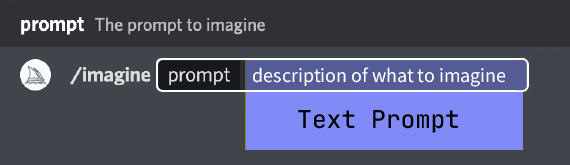
\includegraphics[width=0.475\textwidth]{resources/figures/midjourney_prompts.png}
    \caption{Příkaz pro generování obrázku pomocí Midjourney\cite{midjourney}}
    \label{fig:mj_prompts}
\end{figure}

Tento proces je však také možné obrátit. Modelu je možné poslat obrázek ve formě odkazu. Ten je následně zanalyzován a na základě něj je vygenerován několik textových popisů, které by měly daný vstup vystihnout. Tento způsob je velmi užitečný v případech, kdy chce uživatel použít pouze určité části, či kvality daného obrázku jako předlohu pro generování dalších. Midjourney je také schopno přímo ze vstupních obrázků vygenerovat obrázky nové. V tomto případě však bere model v potaz celý obrázek, což může být v některých případech nežádoucí.

Mimo promptů lze modelu předat i parametry, které dále alterují výstup. Ty se označují dvěma pomlčkami před samotným parametrem. Velmi užitečným se jeví být parametr 'no' pro negativní prompty. To jsou takové prompty, které modelu říkají, co by obrázek neměl obsahovat. Dále lze však využít parametry jako 'style', který mění styl obrázku, či 'cref', díky kterému lze do výsledku přidat konkrétní postavu v různých kompozicích. Tímto způsobem je možné přesněji specifikovat a ovlivnit požadovaný výstup. Celý vstupní řádek je možné vidět na obrázku \ref{fig:mj_prompts_params}.

\begin{figure}[H]
    \centering
    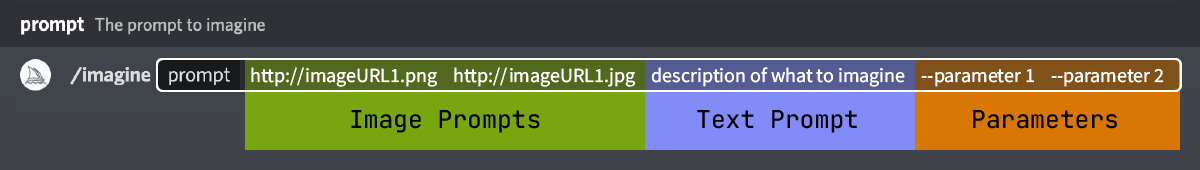
\includegraphics[width=1\textwidth]{resources/figures/midjourney_prompts_params.png}
    \caption{Příkaz pro generování obrázku pomocí Midjourney s parametry\cite{midjourney}}
    \label{fig:mj_prompts_params}
\end{figure}

\subsection{Předčítání textu}
Pro tento účel by bylo možné využít některý z text-to-speach nástrojů, jejichž zdrojové kódy jsou dostupné online. Tyto nástroje jsou schopny přečíst text, který je jim zadán a pomocí algoritmů a neuronových sítí generovat věrnou napodobeninu lidského hlasu. Výhodou těchto nástrojů je, že jsou schopny přečíst texty v mnoha jazycích a že jsou schopny generovat hlas, který zní velmi přirozeně.

Z časových důvodů bylo rozhodnuto, že tato funkcionalita nebude do aplikace implementována, avšak by mohla být v budoucnu přidána jako rozšíření.